
\onecolumn
\begin{inctext}[paper=graphics]
  \begin{tikzpicture}
    \coordinate (below left) at (0in,0in);
    \coordinate (above right) at (8.5in,11in);
    \path[use as bounding box] (below left) rectangle (above right);
    \draw[very thin, Seashell2] (below left) grid (above right);
    \draw (0,25) node[right]
      {\fontsize{100pt}{0pt}\selectfont
        \textbf{Math\textit{\textcolor{DodgerBlue2}{P}}robs}};
    \foreach \pos/\char in {21/数,17.5/学,14/题,10.5/集} {
      \draw (0,\pos) node[right]
        {\fontsize{100pt}{0pt}\selectfont \textbf{\textit{\char}}}; }
    \fill[DeepSkyBlue2] (17.5,23.9) rectangle (22,25.5);
    \fill[DarkSlateGray3] (10,0) -| (22,8) -- cycle;
    \draw (21.5,3) node[left]
      {\fontsize{60pt}{0pt}\selectfont
      \textcolor{DarkSlateGray1}{\textbf{\texttt{0040}}}};
    \draw (21.5,1) node[left]
      {\fontsize{60pt}{0pt}\selectfont
      \textcolor{DarkSlateGray1}{\textbf{-- \texttt{007F}}}};
    \draw (17.5,24.7) node[right] {
      \begin{minipage}{10cm}
        \fontsize{10pt}{10pt}\selectfont \textcolor{Azure1}
        {Copyright \copyright\ 2024 \\
          \textbf{Liu One} \\ \emph{All rights reserved.}}
      \end{minipage} };
    \draw (0,6.9) node[right] {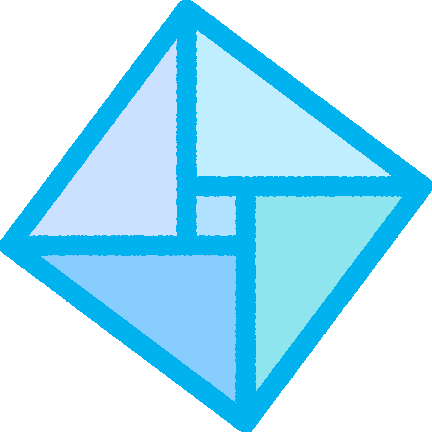
\includegraphics[scale=.45]{covers/logo}};
    \draw (2,4) node {\Huge\textcolor{RoyalBlue1}{\textbf{VOL.}}};
    \draw (2,2) node
      {\fontsize{100pt}{0pt}\selectfont\textcolor{RoyalBlue2}{\textbf{2}}};
    \draw (15,18) node {
      \begin{minipage}{2cm}
        \footnotesize \textit{
        \raggedright 射影几何 \\
        \raggedleft ——发散到无穷,却又汇集于一点 \\ }
      \end{minipage} };
    \begin{scope}[shift={(10,9)}, scale=.9, very thick]
      \coordinate[label=left:$A$] (A) at (0,8);
      \coordinate[label=below:$B$] (B) at (-6,0);
      \coordinate[label=below:$C$] (C) at (3,0);
      \coordinate[label=above right:$D$] (D) at ($ (A)!(B)!(C) $);
      \coordinate[label=above left:$E$] (E) at ($ (A)!(C)!(B) $);
      \path[name path=BD] (B) -- (D);
      \path[name path=CE] (C) -- (E);
      \coordinate[label=below:$U$] (rtBDC) at ($ (B)!(D)!(C) $);
      \coordinate[label=below:$V$] (rtBEC) at ($ (B)!(E)!(C) $);
      \path[name path=DF] (D) -- (rtBDC);
      \path[name path=EG] (E) -- (rtBEC);
      \path[name intersections={of=BD and CE}]
        coordinate[label=above:$O$] (O) at (intersection-1);
      \path[name intersections={of=CE and DF}]
        coordinate[label=above right:$F$] (F) at (intersection-1);
      \path[name intersections={of=BD and EG}]
        coordinate[label=above left:$G$] (G) at (intersection-1);
      \path[name path=AP] (A) -- ($ (B)!1.5!(A) $);
      \path[name path=AQ] (A) -- ($ (C)!2!(A) $);
      \path[name path=DP] (D) -- ($ (F)!5!(D) $);
      \path[name path=EQ] (E) -- ($ (G)!5!(E) $);
      \path[name intersections={of=AP and DP}]
        coordinate[label=above:$P$] (P) at (intersection-1);
      \path[name intersections={of=AQ and EQ}]
        coordinate[label=above:$Q$] (Q) at (intersection-1);
      \coordinate (sec) at ($ (B)!2!(C) $);
      \pic[mark angle={cyan}{2mm}{1}] {right angle=B--E--C};
      \pic[mark angle={cyan}{2mm}{1}] {right angle=B--D--C};
      \pic[mark angle={cyan}{2mm}{1}] {right angle=C--rtBEC--E};
      \pic[mark angle={cyan}{2mm}{1}] {right angle=D--rtBDC--B};
      \fill[opafill=yellow] (E) -- (F) -- (D) -- (G) -- cycle;
      \fill[opafill=green] (E) -- (P) -- (D) -- (Q) -- cycle;
      \draw (A) -- (B) -- (C) -- cycle (B) -- (D) (C) -- (E)
        (D) -- (rtBDC) (E) -- (rtBEC) (A) -- (P) (P) -- (D)
        (A) -- (Q) (P) -- (Q) -- (E);
      \draw[blue] (B) -- (sec) -- (Q) (E) -- (sec) (G) -- (sec);
      \draw[densely dashed, thick, teal] (B) arc (180:0:4.5);
      \draw[very thick, ->] (-6.5,0) -- (4.5,0) node[below] {$x$};
      \draw[very thick, ->] (-1.5,-.5) -- (-1.5,5.5) node[right] {$y$};
    \end{scope}
  \end{tikzpicture}
\end{inctext}
\twocolumn
